Orodja na avtomatih so največkrat narejena iz HSS,
hitroreznega jekla. To so jekla z dodanim kromom, volframom,
molibdenijem, vanadijem in kobaltom. Na splošno skupna količina
legirnih elementov ne presega 7 \%. Trdnost teh jekel je zelo visoka,
od 63 do 67 HRC.

Uporabljajo pa se prav zaradi visoke trdnosti. Z uporabo
brusilnega stroja ali brusilke se surovec obdela v nož po želji,
moramo pa paziti, da pri brušenju jekla ne pregrejemo, saj tako
hitro zgubi svojo trdoto.
Iz njih lahko naredimo katero koli orodje; stružne, odrezne,
profilne nože, kot tudi topovske svedre in pestiče. Surovci so
največkrat dolgi 200 mm in kvadratni s standardnimi merami
(8 x 8, 10 x 10, 12 x 12, 16 x 16 …). Na spodnji Sliki \ref{hss_nozi}
so prikazani HSS-surovci, ki imajo navadno že brušene
nekatere površine za lažje nadaljno brušenje.

\begin{figure}[H]
	\begin{center}
		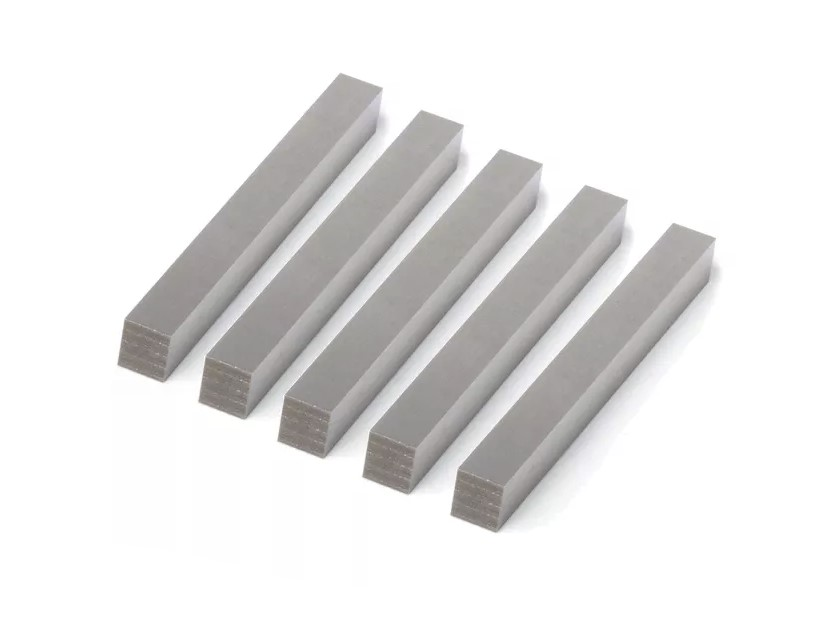
\includegraphics[width=10cm]{hss_nozi.jpg}
		\caption{HSS-surovci
			\cite{hss_nozi}}
		\label{hss_nozi}
	\end{center}
\end{figure}

Obstojnost hitroreznih jekel v primerjavi z ostalimi ni najboljša,
lahko pa se izboljša z raznimi prevlekami. Zaradi teg, se za
avtomatna jekla uporablja večinoma HSS, za trša jekla, nerjavna
in poboljšana pa se uporabljajo noži iz karbidnih trdnin,
narejenih s postopkom sintranja ali WIDIA, ki pa je zelo trda
kovinska zlitina, katere ime je izpeljano iz besed "Wie Diamant",
kar po slovensko pomeni \textit{kot diamant}.

\subsubsection{Rezalna hitrost}
Rezalna hitrost je odvisna od materiala, ki ga obdelujemo,
obdelovalnega postopka, prereza odrezka, hitrosti podajanja
in željene površine (groba ali fina). Vrednosti rezalne hitrosti
najdemo v tabelah, ki so bile narejene na podlagi preizkušanja,
in je nikoli ne računamo. Spodaj na Sliki \ref{rezalna_hitrost}
je primer tabele rezalnih hitrosti, vzetih iz Krautovega strojniškega
priročnika.

\begin{figure}[H]
	\begin{center}
		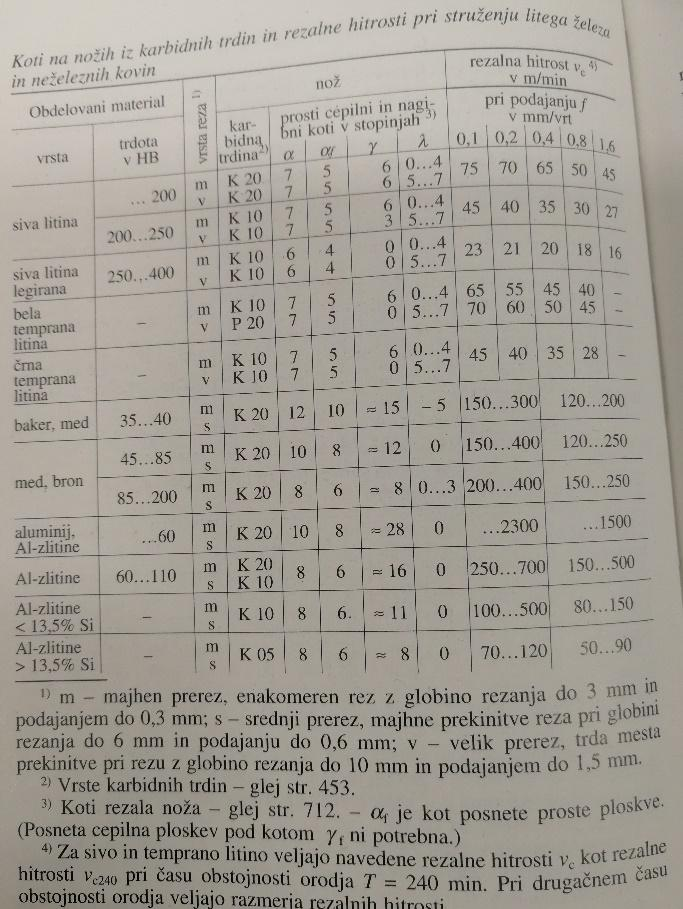
\includegraphics[width=10cm]{rezalne_hitrosti.jpg}
		\caption{Tabela rezalnih hitrosti
			\cite{strojniski_prirocnik}}
		\label{rezalna_hitrost}
	\end{center}
\end{figure}

To rezalno hitrost \(V_c\) nato uporabimo v enačbi
\begin{equation}
	\begin{split}
		V_c &= \frac{\pi*D*n}{1000},
	\end{split}
\end{equation}
kjer je \(D\) premer obdelave in lahko izpostavimo obrate glavnega
vretena \(n\) v \(\frac{obr}{min}\) kot
\begin{equation}
	\begin{split}
		n &= V_c * \pi * D * 1000,
	\end{split}
\end{equation}
nato lahko izračunamo hitrost pomika orodja \(f\) v \(\frac{mm}{min}\):
\begin{equation}
	\label{pomik_orodja}
	\begin{split}
		f &= n * f_z * Z,
	\end{split}
\end{equation}
kjer je:
\begin{itemize}
	\item[--] \(f_z\) -- pomik orodja na en zob in
	\item[--] \(Z\) -- število zob.
\end{itemize}
Pomik na zob \(f_z\) izračunamo z
\begin{equation}
	\label{pomik_na_zob}
	\begin{split}
		f_z &= \frac{f}{n * Z}.
	\end{split}
\end{equation}
Vidimo, da sta \eqref{pomik_orodja} in \eqref{pomik_na_zob} druga od
druge odvisni, zato največkrat sami izberemo \(f_z\) glede na to,
kako togo orodje in stroj imamo ter kakšen material obdelujemo.
Za mehkejše in lažje obdelovalne materiale izberemo večji \(f_z\),
za trdnejše pa manjšega. Pomik na zob izbiramo tudi glede na vrsto obdelave,
če gre za fino obdelavo, kjer so zahtevnejše tolerance in je zahtevana
hrapavost površine, vzememo primerno manjše vrednosti.